%Prílohy

\chapter{Plagát}
\begin{figure}[ht]
\centering
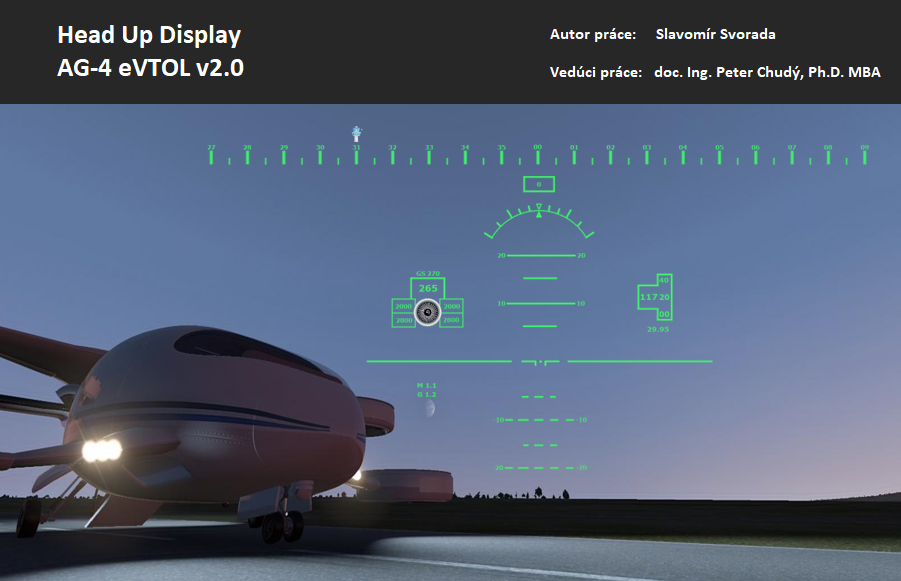
\includegraphics[scale=0.6]{obrazky-figures/plagatFinal.png}
\caption{Plagát prezentujúci priehľadový displej.}{\label{plagat}}
\end{figure}

\chapter{Dotazník k testovaniu}

\noindent

\begin{enumerate}
\item{Aký je Váš vek? \newline
\_\_\_\_\_\_\_\_\_\_\_\_\_\_\_\_\_\_\_\_\_\_\_\_\_\_\_\_\_\_\_\_\_\_\_\_\_\_\_\_\_\_\_\_\_}

\item{Koľko hodín máte nalietaných na leteckom simulátore? \newline
\_\_\_\_\_\_\_\_\_\_\_\_\_\_\_\_\_\_\_\_\_\_\_\_\_\_\_\_\_\_\_\_\_\_\_\_\_\_\_\_\_\_\_\_\_}

\end{enumerate}

\newcolumntype{P}{>{\centering\arraybackslash}p{0.6cm}}
\newcolumntype{L}{>{\raggedright\arraybackslash}m{0.2\textwidth}}
\newcolumntype{R}{>{\raggedleft\arraybackslash}m{0.2\textwidth}}

\newcommand{\printtblhdr}{%
  \hfill
  \begingroup
  \setlength\tabcolsep{0pt}%
  \begin{tabularx}{0.41\textwidth}{ @{} l *{3}X r @{} }
    \multicolumn{2}{l}{\bfseries\shortstack[l]{Zlá}}
    &&
    \multicolumn{2}{l}{\bfseries\shortstack[r]{Výborná}}
    \\
  \end{tabularx}
  \endgroup
}

\newcommand{\usetbl}{%
  \begin{tabular}{ c c c c c c c c c c}
    \hline
    1 & 2 & 3 & 4 & 5 & 6 & 7 & 8 & 9 & 10\\
    \hline
  \end{tabular}
}

\newcommand\prop[1]{%
  \item
  \parbox[t]{0.47\textwidth}{#1}%
  \qquad
  \parbox[t]{0.53\textwidth}{\usetbl}%
}

\printtblhdr

\begin{enumerate}
\setcounter{enumi}{2}
\prop{Aká je čitateľnosť rýchlomera?}

\prop{Aká je čitateľnosť ťahu propulzorov?}

\prop{Aká je čitateľnosť ľavého datového bloku?}

\prop{Aká je čitateľnosť výškomera?}

\prop{Aká je čitateľnosť stupnice klopenia?}

\prop{Aká je čitateľnosť stupnice klonenia?}

\prop{Aká je čitateľnosť stupnice smeru (kurzu)?}


\end{enumerate}
%-----------------------------------------------------------------

\newcolumntype{P}{>{\centering\arraybackslash}p{0.6cm}}
\newcolumntype{L}{>{\raggedright\arraybackslash}m{0.2\textwidth}}
\newcolumntype{R}{>{\raggedleft\arraybackslash}m{0.2\textwidth}}

\newcommand{\printtblhdrr}{%
  \hfill
  \begingroup
  \setlength\tabcolsep{0pt}%
  \begin{tabularx}{0.41\textwidth}{ @{} l *{3}X r @{} }
    \multicolumn{2}{l}{\bfseries\shortstack[l]{Nepáči}}
    &&
    \multicolumn{2}{l}{\bfseries\shortstack[r]{Páči}}
    \\
  \end{tabularx}
  \endgroup
}

\newcommand{\usetbll}{%
  \begin{tabular}{ c c c c c c c c c c}
    \hline
    1 & 2 & 3 & 4 & 5 & 6 & 7 & 8 & 9 & 10\\
    \hline
  \end{tabular}
}

\newcommand\propp[1]{%
  \item
  \parbox[t]{0.47\textwidth}{#1}%
  \qquad
  \parbox[t]{0.53\textwidth}{\usetbll}%
}

\printtblhdrr

\begin{enumerate}
\setcounter{enumi}{9}
\propp{Ako sa Vám páči celková štruktúra HUD?}

\end{enumerate}

%---------------------------------------------------------
\newcommand{\printtblhdrrr}{%
  \hfill
  \begingroup
  \setlength\tabcolsep{0pt}%
  \begin{tabularx}{0.41\textwidth}{ @{} l *{3}X r @{} }
    \multicolumn{2}{l}{\bfseries\shortstack[l]{Zložité}}
    &&
    \multicolumn{2}{l}{\bfseries\shortstack[r]{Jednoduché}}
    \\
  \end{tabularx}
  \endgroup
}

\newcommand{\usetblll}{%
  \begin{tabular}{ c c c c c c c c c c}
    \hline
    1 & 2 & 3 & 4 & 5 & 6 & 7 & 8 & 9 & 10\\
    \hline
  \end{tabular}
}

\newcommand\proppp[1]{%
  \item
  \parbox[t]{0.47\textwidth}{#1}%
  \qquad
  \parbox[t]{0.53\textwidth}{\usetblll}%
}

\printtblhdrrr

\begin{enumerate}
\setcounter{enumi}{10}
\proppp{Aké bolo lietanie na letúne pomocou HUD?}

\end{enumerate}

%--------------------------------------
\begin{enumerate}
\setcounter{enumi}{11}
\item{Obsahoval HUD všetky potrebné časti na vykonanie požadovaných manévrov? \newline
\_\_\_\_\_\_\_\_\_\_\_\_\_\_\_\_\_\_\_\_\_\_\_\_\_\_\_\_\_\_\_\_\_\_\_\_\_\_\_\_\_\_\_\_\_}
\item{Čo sa Vám na HUD najviac páčilo? \newline
\_\_\_\_\_\_\_\_\_\_\_\_\_\_\_\_\_\_\_\_\_\_\_\_\_\_\_\_\_\_\_\_\_\_\_\_\_\_\_\_\_\_\_\_\_}
\item{Čo sa Vám na HUD najviac nepáčilo? \newline
\_\_\_\_\_\_\_\_\_\_\_\_\_\_\_\_\_\_\_\_\_\_\_\_\_\_\_\_\_\_\_\_\_\_\_\_\_\_\_\_\_\_\_\_\_}
\item{Čo by ste prípadne na HUD upravili alebo doplnili? \newline
\_\_\_\_\_\_\_\_\_\_\_\_\_\_\_\_\_\_\_\_\_\_\_\_\_\_\_\_\_\_\_\_\_\_\_\_\_\_\_\_\_\_\_\_\_}
\end{enumerate}

\chapter{Obsah priloženého pamäťového média}
\begin{DESCRIPTION}
  %\item [data/] - dátové sady použité v experimentoch 
  \item [doc/] - zdrojové súbory tohto textu
  \item [src/] - zdrojové súbory implementovaného priehľadového displeja
  \item [poster/] - plagát prezentujúci priehľadový displej
  \item [video/] - video priehľadového displeja
  \item [BP.pdf] - elektronická verzia tohto textu
\end{DESCRIPTION}